\chapter{Metodologie usate e raffinamenti successivi}

\section{Metodologia Agile}

L'intero ciclo di vita del software è stato gestito adottando una metodologia \emph{Agile}.

I metodi Agile sono tali da coinvolgere il più possibile il committente, dando quindi vita a un processo di tipo adattativo: cioè che si adatta alle esigenze del cliente, che possono cambiare durante lo sviluppo.
L'Agile è un processo costituito da finestre di tempo limitate (2-4 settimane) chiamate iterazioni, le quali sono a loro volta scomposte nelle fasi di progettazione, di sviluppo e di test.

\begin{figure}[htbp]
\centering
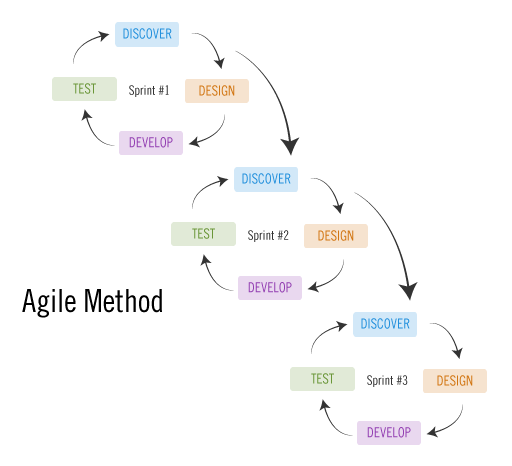
\includegraphics[scale=0.6]{immagini/agile.png}
\caption{Iterazioni e fasi della metodologia Agile}
\end{figure}

Il progetto è quindi suddiviso in singoli componenti indipendenti dalle funzionalità così da poterne analizzare e valutare i costi e i tempi. Ogni iterazione conterrà quindi tutto ciò che è indispensabile per rilasciare un piccolo incremento nelle funzionalità del software e sono tali da essere soggette a modifiche al fine di migliorare l'architettura finale del software.
% Anche se in un'iterazione non si hanno sufficienti funzionalità per ottenere un componente completo, esso deve esser rilasciato e nelle iterazioni successive dovrà avvicinarsi alle richieste del cliente.
% 
% Anche se il risultato di ogni singola
% iterazione non ha sufficienti funzionalità da essere considerato completo,
% deve essere rilasciato e nel susseguirsi delle iterazioni, deve avvicinarsi
% sempre di più alle richieste del cliente. Alla fine di ogni iterazione il team
% dovrà rivalutare le priorità del progetto.
% 
% Ogni iterazione è progetto a sé
% stante e deve contenere tutto ciò che è necessario per rilasciare un piccolo
% incremento nelle funzionalità del software: pianificazione (user stories),
% design, implementazione, test. An
% 
% Sulla scorta di queste considerazioni, nelle metodologie agili i vincoli principali dei progetti
% diventano i tempi, i costi e la possibilità di favorire la gestione del cambiamento dei requisiti.
% Naturalmente, per poter operare in tal modo, è richiesta la suddivisione in singoli componenti
% indipendenti delle funzionalità, al fine di poterne valutare i tempi, i costi e la possibilità di
% completarli procedendo per piccoli incrementi progressivi. In tal modo, viene agevolata anche la
% suddivisione dei compiti e delle responsabilità ai componenti del team di sviluppo.
% In definitiva, i Metodi Agili [21] sono un insieme di tecniche di sviluppo software che si
% focalizzano sullo sviluppo ed il rilascio incrementale (ed in tempi brevi) di porzioni del sistema, che
% siano usabili.
% 
% 
% 
% A differenza delle metodologie "pesanti", quelle agili sono caratterizzate da un processo
% iterativo scomposto in fase di progettazione, di sviluppo e test96 di breve durata.
% Tipicamente, i Metodi Agili si basano su di una disciplina rigorosa che dà vita ad un processo
% ben definito; si noti, però, che quest'ultimo è di tipo adattativo: si adatta, cioè, alle esigenze del
% committente, che possono mutare durante lo sviluppo. Quest'ultimo di focalizza su gruppi di
% funzionalità ed è guidato dalla necessità di rilasciare prodotti di progetto usabili.
% Dunque, gli artefatti possono considerarsi "leggeri", cioè manca la "pesante" documentazione.
% Il lavoro di progettazione, anzichè essere concentrato nella sola parte iniziale, è continuo e
% distribuito lungo tutte le fasi del processo. Pertanto, anche le parti già realizzate sono soggette a
% modifiche, al fine di migliorare l'architettura del software.
% 
% 
% Da ultima troviamo le metodologie agili. Questo particolare metodo di
% sviluppo software, a differenza dei precedenti, coinvolge quanto più
% possibile il committente, ottenendo in tal modo un elevata reattività alle
% sue richieste.
% La gran parte dei metodi agili tentano di ridurre il rischio di fallimento
% sviluppando il software in finestre di tempo limitate chiamate iterazioni
% che in genere durano qualche settimana. Ogni iterazione è progetto a sé
% stante e deve contenere tutto ciò che è necessario per rilasciare un piccolo
% incremento nelle funzionalità del software: pianificazione (user stories),
% design, implementazione, test. Anche se il risultato di ogni singola
% iterazione non ha sufficienti funzionalità da essere considerato completo,
% deve essere rilasciato e nel susseguirsi delle iterazioni, deve avvicinarsi
% sempre di più alle richieste del cliente. Alla fine di ogni iterazione il team
% dovrà rivalutare le priorità del progetto.
% 
% Un'importante constatazione che ha spinto verso questo approccio riguarda la natura mutevole
% nel tempo dei requisiti di un progetto. Pertanto, nell'ottica della pianificazione delle attività, i
% requisiti iniziali potrebbero risultare un punto di partenza inadeguato.
% L'adozione di un approccio è strettamente vincolato alla natura dei requisiti utente: del resto,
% sebbene averne cognizione definitiva già dal principio sia un aspetto desiderabile in qualunque
% progetto software, ciò avviene raramente. Inoltre, anche se accadesse, la fase di progettazione
% potrebbe ugualmente presentare qualche difficoltà.

\section{Requisiti funzionali finali}

Una progettazione iterativa e focalizzata sull'utente ha permesso quindi di ampliare e raffinare i requisiti fino ad ottenere  un risultato sempre più vicino alle richieste e alle necessità del committente.  

Per brevità di seguito sono riportati solo alcuni dei requisiti finali del progetto (che vanno ad aggiungersi o a integrare quelli della tabella \ref{tab:requisiti_iniziali}), per comodità raccolti in categorie.
\begin{center}
    \captionof{table}{Requisiti funzionali finali}

    \begin{longtable}{p{6cm}|p{8cm}}

    \toprule
    \multicolumn{1}{c}{\textbf{Requisito funzionale}} &
    \textbf{Descrizione}\\

    \midrule
    Accesso ai servizi & \begin{itemize}
                          \item Permettere l'accesso ai servizi attraverso credenziali
                          \item Permette l'accesso veloce a un sottoinsieme di funzioni salvando le credenziali
                          \item Permettere recupero Codice Cliente
                         \end{itemize}\\\\

    Riepilogo movimenti & \begin{itemize}
                           \item Rappresentare i movimenti di un conto attraverso una timeline
                           \item Mostrare i movimenti di un conto in una lista
                           \item Visualizzare una scheda di dettaglio per un movimento selezionato
                          \end{itemize}\\\\
    Filtro movimenti & Offrire la possibilità di filtrare i movimenti per data e per tipo (entrate, uscite, tutti)\\\\
    Riepilogo conti e carte & \begin{itemize}
				\item Visualizzare i prodotti di un utente attraverso bubble contenenti informazioni di riepilogo
				\item Visualizzare i prodotti di un utente attraverso una lista
				\item Permettere la selezione di un determinato prodotto
                              \end{itemize}\\\\
    Filtro conti e carte & Permettere la visualizzazione o meno di certi prodotti mediante un filtro\\\\
    Storico saldi & Visualizzare in un grafico a bolle lo storico dei saldi di un prodotto per mesi o settimane \\\\
    Disporre operazioni bancarie & \begin{itemize}
				      \item Fornire un form per la compilazione di dispositive 
				      \item Permettere la riproposizione di dispositive già effettuate
				    \end{itemize}\\\\
    Riepilogo dispositive effettuate & \begin{itemize}
                                        \item Visualizzare le ultime $n$ dispositive in una lista ordinata
                                        \item Visualizzare le ultime $n$ dispositive in un grafico a bolle
                                        \item Permettere il salvataggio delle dispositive effettuate in una lista di preferiti
                                       \end{itemize}\\\\
    Preferiti & Permettere la visualizzazione e la modifica di una lista di dispositive scelte come preferite\\\\\
    Rubrica & Permettere l'accesso in lettura e scrittura alla rubrica del dispositivo per poter salvare o recuperare numeri telefonici\\\\
    
    Help e gestore & \begin{itemize}
                      \item Offrire una sezione interna al software in cui l'utente può richiedere appuntamenti con un consulente
                      \item Mettere a disposizione una sezione di help e numeri utili
                     \end{itemize}\\\\

    Integrazione social network & \begin{itemize}
                                   \item Visualizzare i contenuti dei canali social offerti dal committente
                                   \item Offrire la possibilità di condividere i contenuti sui diversi social network
				   \item Integrare un player video per la visualizzazione di filmati relativi alle attività del committente
                                  \end{itemize}\\
     Browsing interno & Permettere la navigazione tra contenuti web attraverso un browser interno all'applicazione\\\\
     Notifiche Push & Permettere la ricezione di notifiche push\\\\
     Messaggistica		 & \begin{itemize}
                                   \item Visualizzare i messaggi ricevuti dai servizi
                                   \item Permettere la gestione dei messagi (esempio: cancella, segna come letto, ecc\dots)
                                  \end{itemize}\\
    \bottomrule

    \end{longtable}
\end{center}


\newpage

Sono inoltre elencati alcuni dei requisiti non funzionali:

\begin{center}
    
    \captionof{table}{Requisiti non funzionali}

    \begin{tabular}{p{6cm}|p{8cm}}

    \toprule
    \multicolumn{1}{c}{\textbf{Requisito non funzionale}} &
    \textbf{Descrizione}\\

    \midrule
    Comunicazione sicura & \begin{itemize}
                            \item Garantire la comunicazione sicura tra client e server
                            \item Garantire che i dati salvati all'interno del device siano protetti
                           \end{itemize}\\\\
    Ottimizzazione flusso dati & Limitare il più possibile il consumo dei dati\\\\
    Efficienza & Garantire uso efficiente delle risorse offerte dal device (cpu, batteria, ecc\dots)\\

    \bottomrule

    \end{tabular}
%     \label{tab:requisiti_non_funz}

\end{center}

